\chapter{Research Design}
\label{ch:researchDesign}
\section{Overall plan}
\label{sec:overview}
%I would like to include the name or section where this method is used, but I am not sure where to exactly put it. I guess I can put it into the sections that justify and talk about the method. 
% REVIEW: What does this even mean? ^

This section provides an overview of how our chosen research methods relate to each other and how they assist in answering the research questions we have posed. Table~\ref{tab:designPlan} gives a quick overview of our methods and which specific research question the method contributes to. The table order corresponds to when in our project the research method was used.

The first research question is concerned with finding relevant scenarios for the use of systems such as the one we are creating. To answer this question we preformed interviews and focus groups. A large part of the second focus group was dedicated to discussing different scenarios with the physiotherapists.

The second research question asks what functional and user experience requirements the visualizations should have. The initial requirements were gathered through an interview with a domain expert. Two revisions of the requirements were planned, one after each focus group. Feedback on the prototype was the basis for the modifications to the requirements. A portion of the second focus group was used to discuss the requirements with the physiotherapists.

Research question 3 asks which visualizations the physiotherapists prefer, given the requirements and scenarios created. Feedback on the visualizations was given in the focus groups. The larger part of both focus groups was planned for discussing and reviewing the visualizations with the physiotherapists. 

\begin{table}[h!]
  \centering
  \begin{tabular}{|p{0.7cm}|p{2cm}|p{9cm}|}
    \hline
    \textbf{RQ} & \textbf{Method} & \textbf{Description} \\ \hline
    1,2 & Interview & An interview was performed with a domain expert which would allows us to establish initial requirements. \\ \hline
    2 & Brainstorming & Based on the initial requirements the authors performed brainstorming sessions among themselves and sketches were created. \\ \hline
    2, 3 & Prototype & The paper sketches were used as a starting point to create a high fidelity prototype that would be presented to first focus group. \\ \hline
    1,2,3 & Focus group & The first running prototype was presented to the focus group and would enable us to refine it further. \\ \hline
    2, 3 & Prototype & Based on the feedback received from the first focus group the prototype was iterated. \\ \hline
    None & Questionnaire & Before the final focus group a quick questionnaire was answered by the users. \\ \hline
    1,2,3 & Focus Group & The new iteration of the prototype was presented and the requirements were refined. \\ \hline
    1,2 & Interview & At the end an interview was carried out to help us understand how the physiotherapists work. \\ \hline
  \end{tabular}
  \caption{The overall design plan}
  \label{tab:designPlan}
\end{table}

More detailed information about how the methods were executed and their result can be found in the subsequent chapters of this report, namely in Chapter 6 to 10. The following sections of this Chapter explain the rationale and choice of method in further detail.
 
\section{Overall plan in accordance to ISO}
This subsection aims to show how our chosen research methods relate to human-centred design activities describes in ISO 9241-210. Figure~\ref{fig:hcdActivitiesOurs} show how our research methods correspond to the ISO activities. The gray text is the purpose of the step described in ISO 9241-210, inside of the squares are our research methods with an numbering showing the order in which they were executed. The Brainstorming and Questionnaire activities have been omitted from the figure, they were primarily used as support methods for prototype 1 and focus group 2.

\begin{figure}[h!]
	\centering
		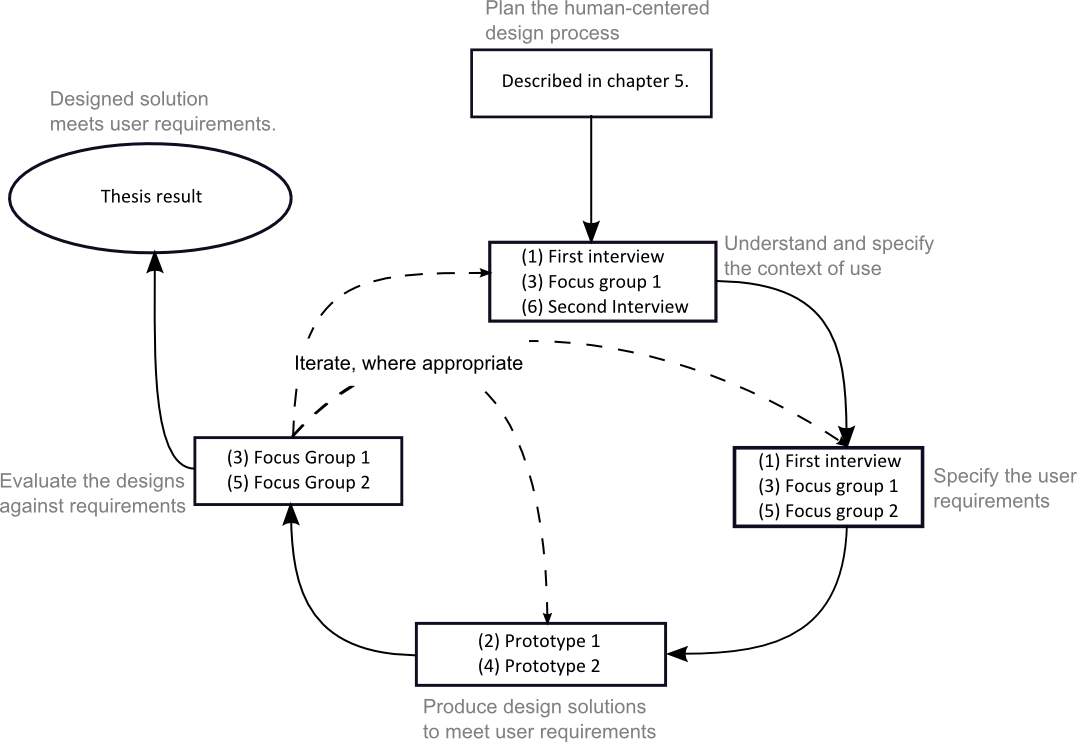
\includegraphics[width=0.9\textwidth]{hcdActivitiesOurs.png}
		\caption{\footnotesize H}
		\label{fig:hcdActivitiesOurs}
\end{figure}

\section{Interview}
Initially we had no domain knowledge or experience with how visualizations should be used to present sensor data. So when the time came to outline initial requirements and scenarios we anticipated that we would require assistance. While attempting to acquire a set of activPAL sensor from St. Olav's Hospital we came in contact with a physiotherapist and PhD candidate who had extensive knowledge about activPAL and experience in visualization of sensor data. 

We considered performing a field study, a focus group or an interview. In the end we chose to interview the domain expert. We believed that a field study and focus group would not be fruitful enough to justify the amount of time it would take. We lacked a grasp of basic knowledge and terminology in the field that could be covered by a simple interview, without being confused or influenced by the multitude of opinions that would appear in a focus group or field study. The procedure and results of this interview can be found in chapter~\ref{ch:initialRequirements}. 

Originally we had intended to conduct a minor literature study to understand how physiotherapy is conducted in Norway. Sadly this was not a well documented process, and the little information we did find was not consistent. The routines varied from office to office, and what type of patients they focused on. Therefore we decided to conduct an interview with some of the participants from the planned focus group. Our summary of this interview can be found in section~\ref{sec:physiotherapyPractice}.
 
\section{Brainstorming}
Jumping straight to a high fidelity prototype would be unwise, therefore we decided that we should conduct brainstorming sessions. The purpose was to create rough designs of possible visualizations that would fulfill the initial requirements, in addition to discussing any technical difficulties that might occur during implementation. In order to verify that the ideas were sound and receive some outside input we had our advisor provide us with feedback on the visualizations. We tried contacting the domain expert, but the individual was not available on such short notice, and we did not wish to wait for too long. The result of the brainstorming can be found in Section~\ref{sec:paperSketches}.

\section{Prototype}
Once we were happy with our paper sketches we decided to start implementing a running prototype. We did not want to spend more time on low fidelity prototypes that would be thrown away at the end, and would most likely never be shown to a broader set of users. A running prototype showing real data and more polished visualizations would have a much bigger impact on the focus group than rough paper sketches. In addition there was a fair amount of technical aspects we were unsure of because we had not created such an application before, so starting development early was important. The first version of the prototype can be seen in section~\ref{sec:runningPrototype1} and the second iteration can be found in section~\ref{sec:runningPrototype2}.

%Review me!
Figure~\ref{fig:hillTrianglePrototypex} shows what type of design questions the paper sketches and running prototypes attempt to answer. The Paper sketches (PS) are a result of the brainstorming session conducted and focus heavily on the \textit{look and feel}, as they were designed with the scenarios and requirements in mind, \textit{role} questions are answered as well. Our first running prototype resolved any implementation uncertainties we had, and in addition helped us solidify our look and feel. Creating the second prototype after a focus group allowed us to refine the look and feel while designing it more role oriented based on the feedback and scenarios presented after the first focus group.

\begin{figure}[h!]
	\centering
		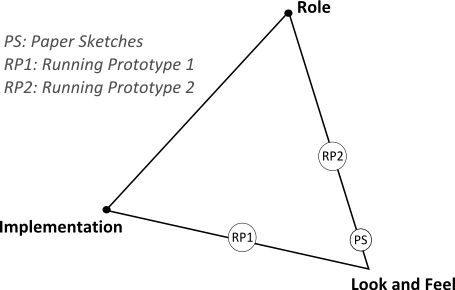
\includegraphics[width=0.7\textwidth]{hillTrianglePrototypes.png}
		\caption{\footnotesize Showing where the focus of our prototypes lie.}
		\label{fig:hillTrianglePrototypex}
\end{figure}

\section{Focus group}
Initially we were uncertain if a focus group should be conducted or usability tests should be run. In the end we decided that the main priority and focus were the visualizations themselves, and the navigation was not of a major concern. A focus group would provide us with the necessary feedback, while taking less time and having the benefit of letting the users discuss the prototype with each other. Detailed information on how the first focus group was conducted can be found in chapter~\ref{ch:focusGroup1} while the second focus group is covered in chapter~\ref{ch:focusGroup2}.

\section{Questionnaire}
A questionnaire was created after the first focus group and presented to the participants of the second focus group. The purpose was to gain more background information about the participants to gain an understanding of their attitude towards technology and if it can help to improve their work. It was decided that it would be best to present the questionnaire during the second focus group. This would allow us to create simple background questions we felt were not answered clearly during the first focus group, but were not important enough to spend time on discussing thoroughly.
